\clearpage{\pagestyle{empty}\cleardoublepage}
\chapter{Visualizzazione dati sull'utilizzo del progetto BolognaWiFi}
In questo capitolo andremo a trattare l'applicazione sviluppata, partendo dall'ambiente di lavoro, con le regole di stile per un codice pulito, e arrivando a esplorarne i principali obiettivi, i problemi affrontati e le soluzioni implementate, mostrando anche qualche schermata dell'applicazione così realizzata.

\section{Il caso studio: dati del BolognaWiFi}
% Descrizione del dataset, valore informativo, applicazioni per la pianificazione e gestione urbana
Il Comune di Bologna offre una serie di Open Data relativi al BolognaWiFi, riguardanti affollamento, affluenza e spostamenti. Questi dati vengono pubblicati ogni giorno in formato JSON e il loro contenuto si riferisce a tutte le entrate giornaliere, riguardo alle varie zone e spostamenti, aggiornate a tre giorni prima della data odierna. Tutti questi dati sono stati aggregati in maniera oraria e anonima, quindi è impossibile risalire ai singoli dispositivi, rispettando così la privacy degli utenti. La struttura dei dati non è omogenea in tutti e tre i dataset, quindi andremo a esplorarla nel dettaglio.


Gli spostamenti, invece, hanno un'entrata per ogni spostamento che viene effettuato in una data ora del giorno, aggregati in maniera oraria e anonima. Quindi, per ogni zona esiste un dato su affollamento e affluenza in una precisa ora, ma lo stesso non può dirsi riguardo agli spostamenti in quanto non è detto che avvengano sempre, ad esempio durante le ore notturne.

\subsection{Spostamenti}
Per gli spostamenti viene registrata una nuova entrata per ogni spostamento che viene effettuato in una data ora del giorno. Non è detto che ad ogni ora del giorno corrisponda almeno uno spostamento da una zona all'altra, in quanto non è detto che avvengano sempre, si pensi ad esempio durante le ore notturne. Tali spostamenti sono direzionati, quindi uno spostamento dalla Biblioteca Salaborsa a Palazzo D'Accursio verrà registrato separatamente da quello effettuato, inversamente, da Palazzo D'Accursio a Biblioteca Salaborsa. Anche in questo caso, entrambe le direzioni degli spostamenti sono indipendenti l'una dall'altra, e non è detto che esistano entrambe in una certa ora. Per esempio, potremmo avere una direzione in cui si spostano 100 persone (o meglio, dispositivi), mentre nell'altra se ne spostano 0 o comunque una quantità trascurabile ai fini del rilevamento dati di BolognaWiFi, quindi in entrambi questi ultimi due casi non verrebbe creata nessuna nuova entrata sul database di Open Data. Questo aiuta anche a garantire la privacy degli utenti, in quanto se venissero pubblicati i dati di un singolo dispositivo in una certa direzione il diritto alla privacy potrebbe venire violato.

\begin{figure}[h]
    \centering
    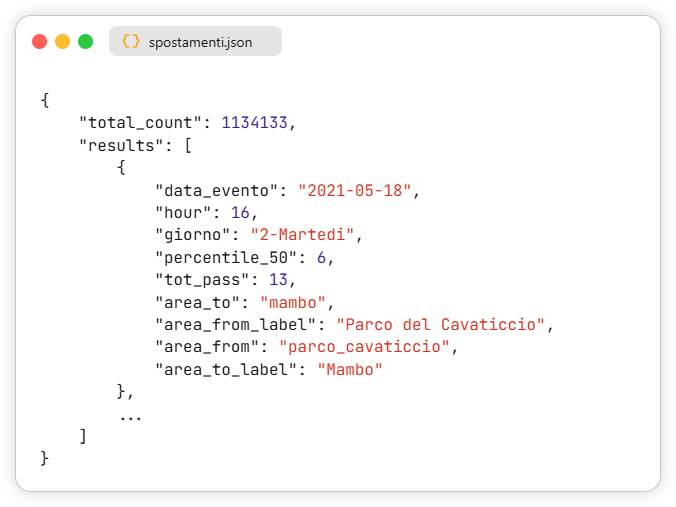
\includegraphics[width=0.75\textwidth]{spostamenti_alt}
    \caption[Struttura dei dati sugli spostamenti]{Dati relativi agli spostamenti, in formato JSON, riferiti ai movimenti da Parco del Cavaticcio a Mambo, alle ore 16 del 18 maggio 2021.}
\end{figure}

\subsection{Affollamento e Affluenza}
Dato che affollamento e affluenza contengono dati aventi una struttura molto simile tra loro, possiamo trattarli insieme. Per entrambi viene registrata una nuova entrata per ogni ora del giorno, in ciascuna zona di Bologna coperta dal servizio BolognaWiFi.

\begin{figure}[H]
    \centering
    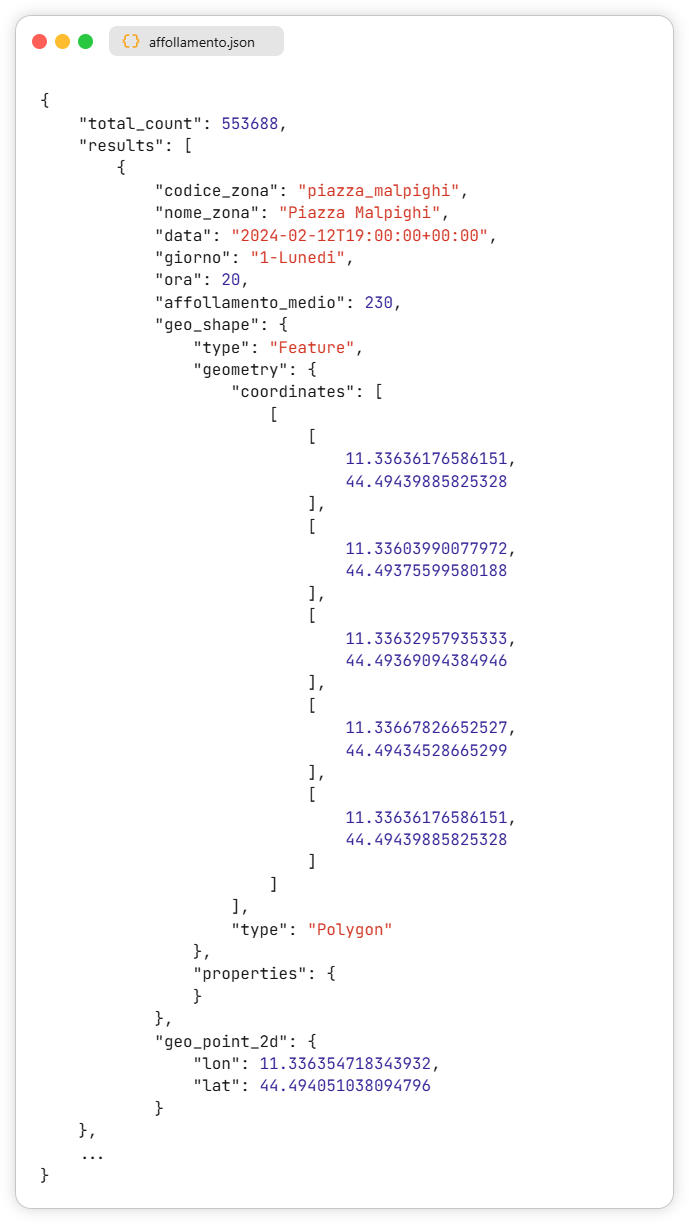
\includegraphics[width=0.75\textwidth]{affollamento_alt}
    \caption[Struttura dei dati sull'affollamento]{Dati riguardanti l'affollamento, in formato JSON, riferiti a Piazza Malpighi alle ore 20 del 12 febbraio 2024. Notare l'attributo \textit{ora} che viene incluso nel timestamp di \textit{data} in fuso orario UTC.}
\end{figure}

\begin{figure}[H]
    \centering
    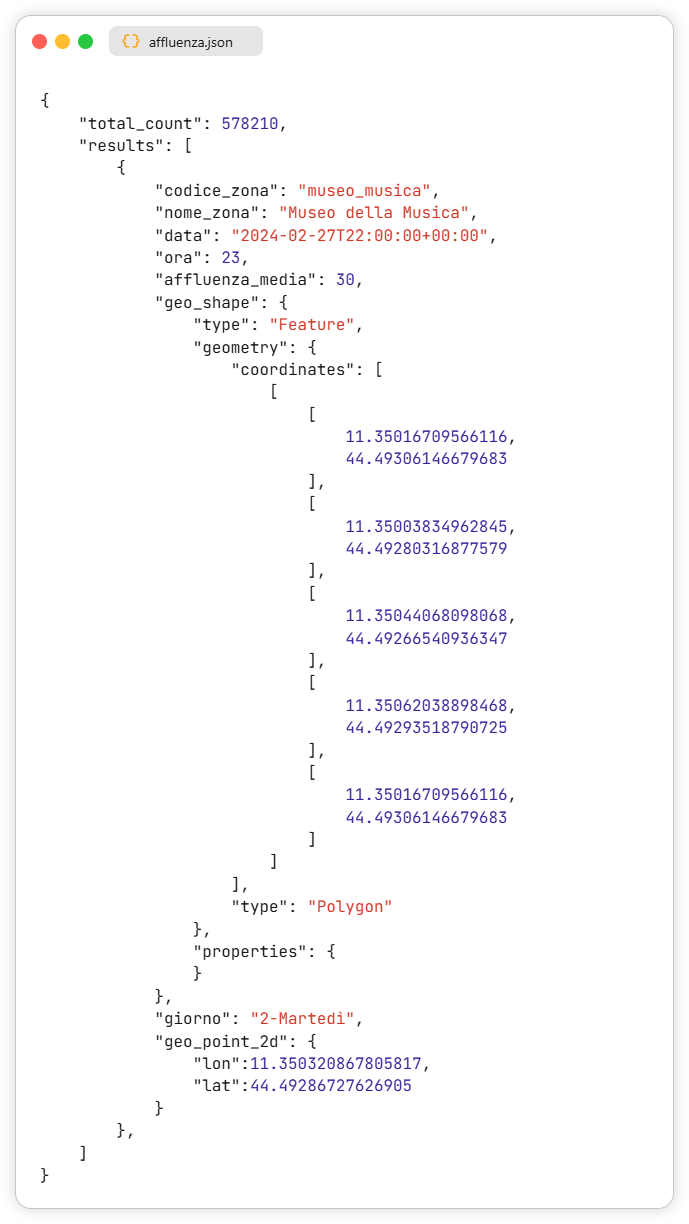
\includegraphics[width=0.75\textwidth]{affluenza_alt}
    \caption[Struttura dei dati sull'affluenza]{Dati riguardanti l'affluenza, in formato JSON, riferiti al Museo della Musica, alle ore 23 del 27 febbraio 2024. Notare l'attributo \textit{ora} che viene incluso nel timestamp di \textit{data} in fuso orario UTC.}
\end{figure}

\section{Struttura del database}
\section{Connessione tra frontend e backend}
\section{Implementazione richieste AJAX}
\section{Popolamento del database}
\section{Single-Page App}
\section{Stile del codice}
\section{Funzionalità}
\section{Informazioni su una zona o spostamento}
\section{Calcolo del colore di una zona}
\section{Raggruppamento dei dati giornalieri}
\section{Questionario SUS sull'esperienza utente}